\definecolor{meuVerde}{RGB}{0, 95, 0}
\definecolor{meuVermelho}{RGB}{127, 0, 0}
\definecolor{meuAzul}{RGB}{0, 0, 191}
\newcommand{\red}[1]{\textcolor{meuVermelho}{#1}}
\newcommand{\green}[1]{\textcolor{meuVerde}{#1}}
\newcommand{\blue}[1]{\textcolor{meuAzul}{#1}}

Simular os turnos do jogo envolveria realizar as somas iterando sobre o tabuleiro $N \times N$ para os $T$ turnos. A complexidade seria $\mathcal{O}(N^2\cdot T$), o que seria impraticável para o tempo limite de 1 segundo.

No entanto, pode-se montar uma matriz que represente a recursão do problema, levando em consideração as escolhas dos jogadores. Nesse caso, é possível utilizar algum algoritmo de exponenciação de matrizes que seja suficientemente rápido. O mais comum é a \href{https://cp-algorithms.com/algebra/binary-exp.html}{exponenciação binária}. Este não será explicado em detalhes aqui, mas consiste em se aproveitar da propriedade associativa da multiplicação de matrizes de uma forma recursiva. Sendo $\mathbf{M}$ uma matriz, pode-se calcular $\mathbf{M}^n$ com $\mathbf{M}^\frac{n}{2}\cdot\mathbf{M}^\frac{n}{2}$ se $n$ for par, ou $\mathbf{M}^{n-1}\cdot\mathbf{M}$ para $n$ ímpar.

Se tiver dificuldade em programar soluções que envolvem operações de matrizes, veja este \href{https://codeforces.com/blog/entry/21189}{recurso}. Toda vez que pensar em uma solução que usa matrizes, é só copiar o código do seu caderno. Isso poupa \textbf{muito} tempo.

Para entender melhor a ideia, usaremos o exemplo dado no enunciado, onde temos o seguinte tabuleiro na entrada, expandido até o caso geral:

\begin{center}
    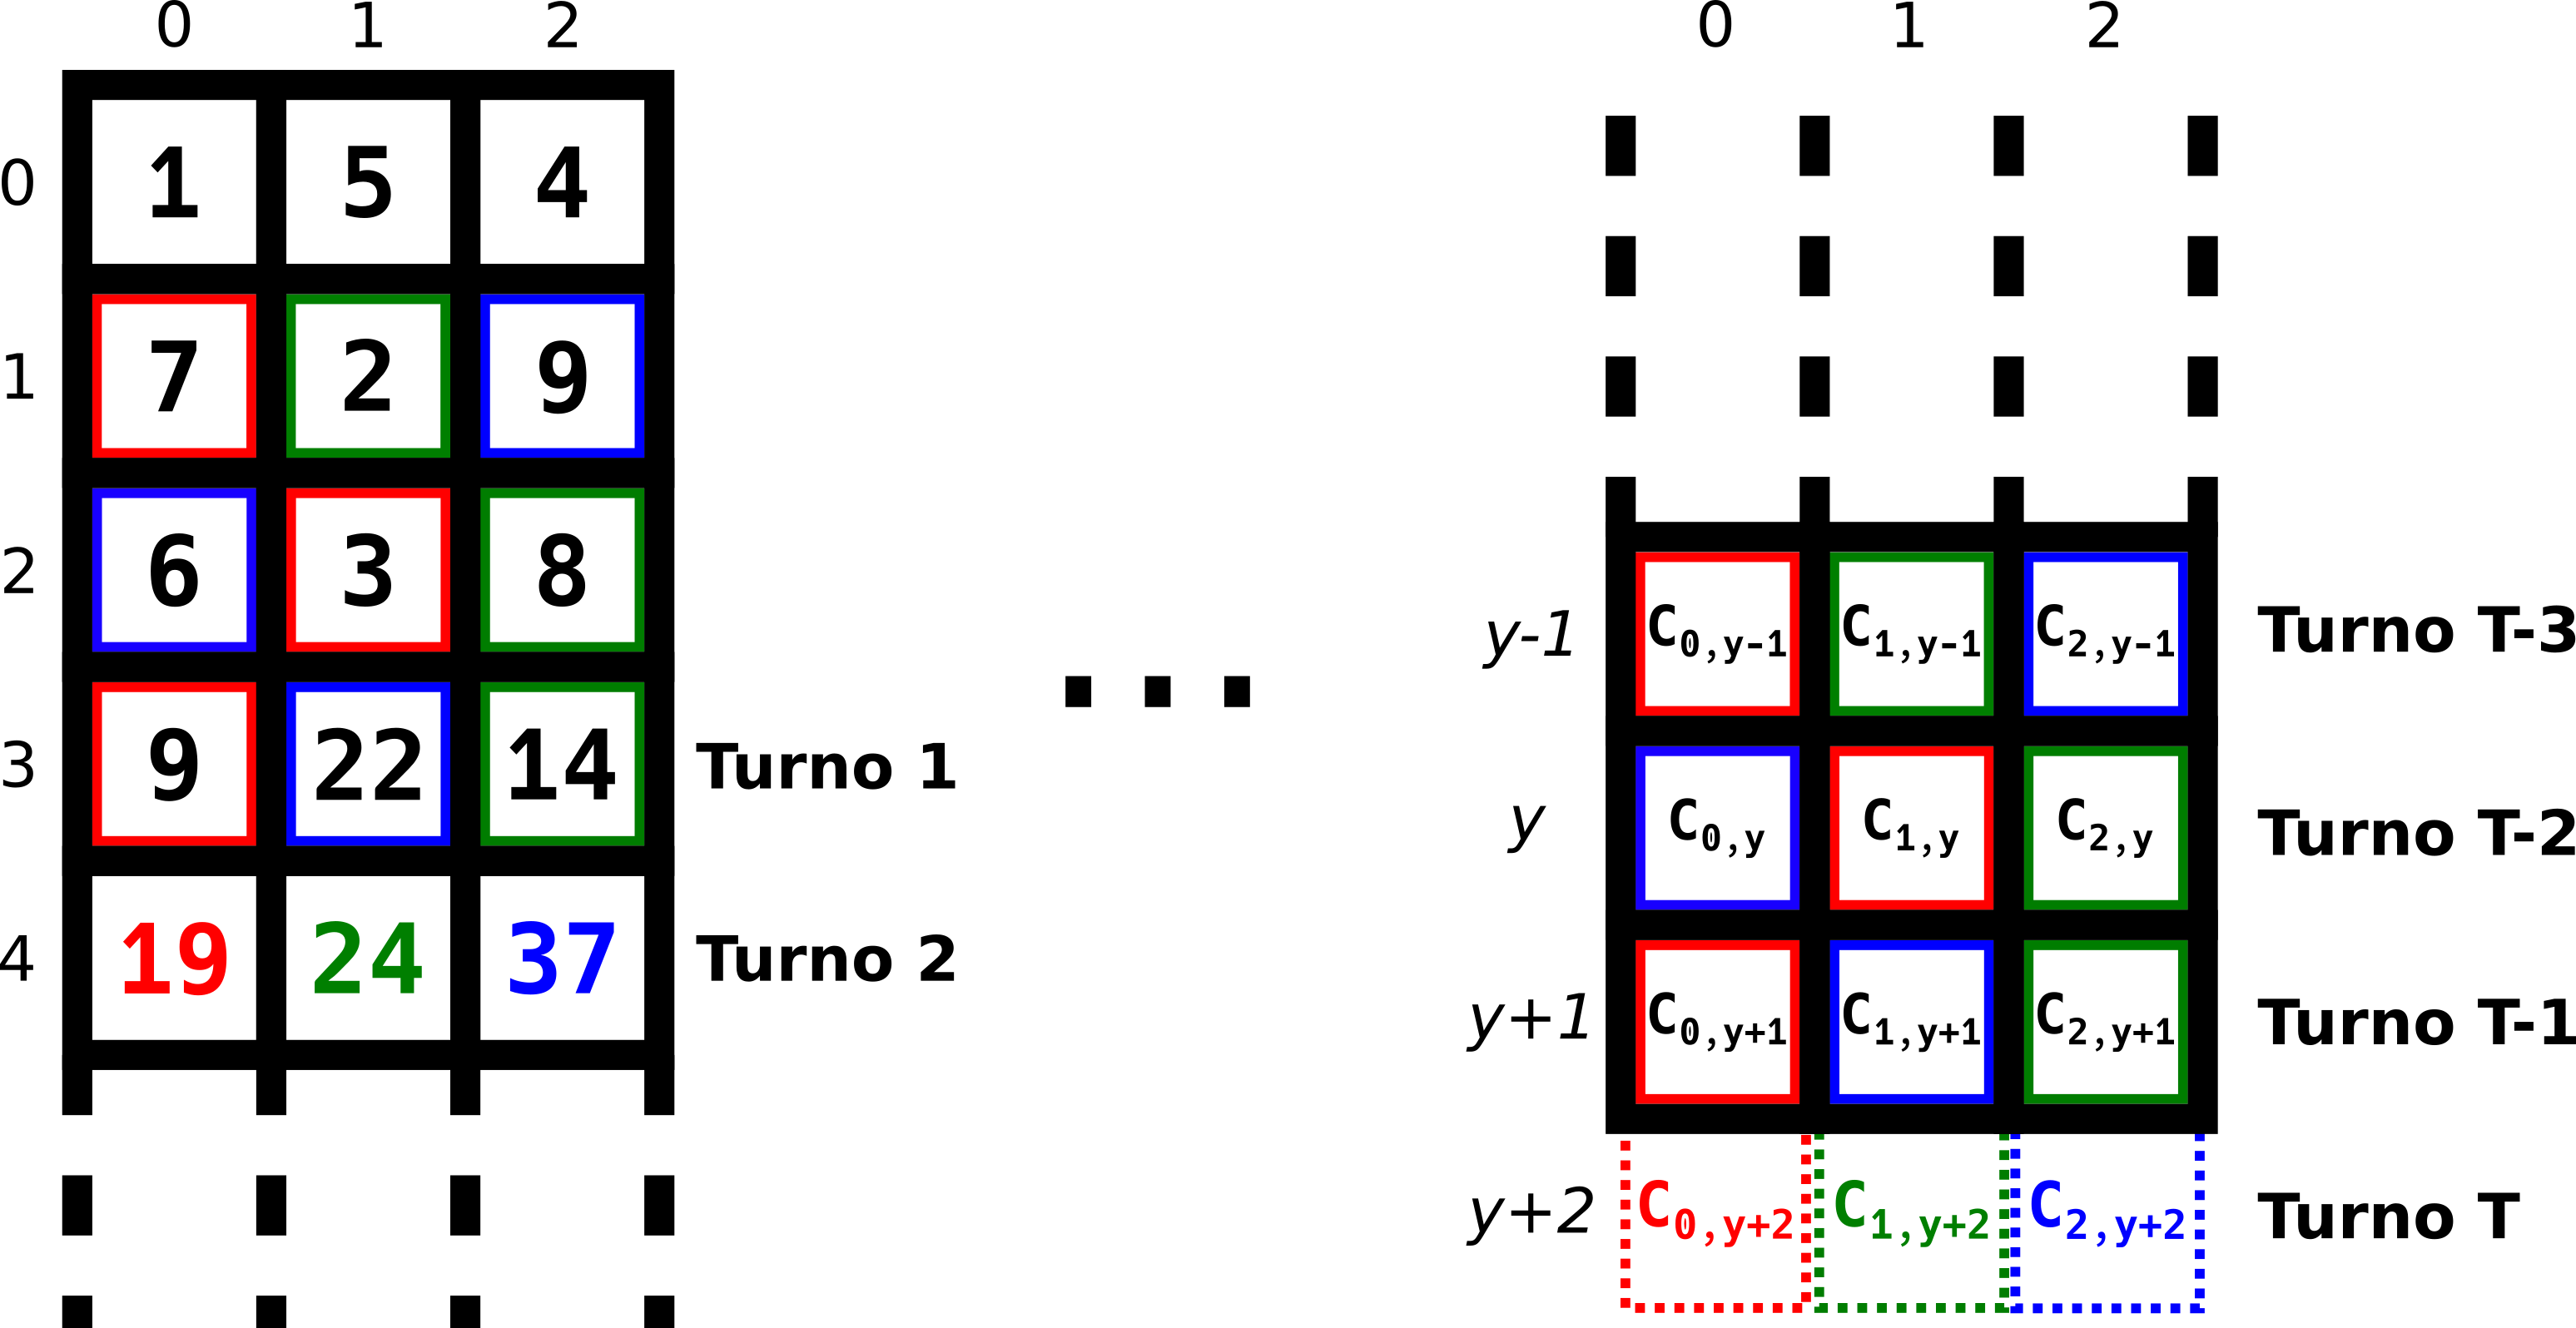
\includegraphics[scale=0.6]{kummirub/exemplo-editorial.png}
\end{center}

Indexando as coordenadas em $x$ e $y$ das casas a partir de $0$, podemos chegar ao seguinte passo recursivo, para quando $y \geq 3$:

\begin{equation}
    \begin{cases}
        \red{C_{0,y+2} = C_{0,y+1} + C_{1,y} + C_{0,y-1}} \\
        \green{C_{1,y+2} = C_{2,y+1} + C_{2,y} + C_{1,y-1}} \\
        \blue{C_{2,y+2} = C_{1,y+1} + C_{0,y} + C_{2,y-1}}
    \end{cases}
\end{equation}

Então, é possível montar a seguinte relação, utilizando matrizes:

\[
\begin{bmatrix}
    \red{C_{0,y+2}} \\ \green{C_{1,y+2}} \\ \blue{C_{2,y+2}} \\ C_{0,y+1} \\ C_{1,y+1} \\ C_{2,y+1} \\ C_{0,y} \\ C_{1,y} \\ C_{2,y}
\end{bmatrix}
=
\begin{bmatrix}
    1&0&0&0&1&0&1&0&0 \\
    0&0&1&0&0&1&0&1&0 \\
    0&1&0&1&0&0&0&0&1 \\
    1&0&0&0&0&0&0&0&0 \\
    0&1&0&0&0&0&0&0&0 \\
    0&0&1&0&0&0&0&0&0 \\
    0&0&0&1&0&0&0&0&0 \\
    0&0&0&0&1&0&0&0&0 \\
    0&0&0&0&0&1&0&0&0
\end{bmatrix}
\begin{bmatrix}
    \red{C_{0,y+1}} \\ \blue{C_{1,y+1}} \\ \green{C_{2,y+1}} \\ \blue{C_{0,y}} \\ \red{C_{1,y}} \\ \green{C_{2,y}} \\ \red{C_{0,y-1}} \\ \green{C_{1,y-1}} \\ \blue{C_{2,y-1}}
\end{bmatrix}
\]

Ao expandir a recursão, chega-se em:

\[
\begin{bmatrix}
    \red{C_{0,y+2}} \\ \green{C_{1,y+2}} \\ \blue{C_{2,y+2}} \\ C_{0,y+1} \\ C_{1,y+1} \\ C_{2,y+1} \\ C_{0,y} \\ C_{1,y} \\ C_{2,y}
\end{bmatrix}
=
\begin{bmatrix}
    1&0&0&0&1&0&1&0&0 \\
    0&0&1&0&0&1&0&1&0 \\
    0&1&0&1&0&0&0&0&1 \\
    1&0&0&0&0&0&0&0&0 \\
    0&1&0&0&0&0&0&0&0 \\
    0&0&1&0&0&0&0&0&0 \\
    0&0&0&1&0&0&0&0&0 \\
    0&0&0&0&1&0&0&0&0 \\
    0&0&0&0&0&1&0&0&0
\end{bmatrix}^{T}
\begin{bmatrix}
    C_{0,2} \\ C_{1,2} \\ C_{2,2} \\ C_{0,1} \\ C_{1,1} \\ C_{2,1} \\ C_{0,0} \\ C_{1,0} \\ C_{2,0}
\end{bmatrix}
\]

Após realizar a exponenciação, basta realizar a multiplicação para obter as respostas esperadas.

Para $N$ jogadores, é necessária uma matriz $N \times N$ como visto no exemplo acima. Assim, a multiplicação de matrizes tem complexidade $\mathcal{O}(N^6)$. Já a exponenciação binária da matriz tem complexidade $\mathcal{O}(\lg(T))$. 

Complexidade total: $\mathcal{O}(N^6 \lg(T))$.
